\documentclass[UTF8]{ctexart}
%%%%%%%%%%%%%%%%%%%%%%%%%%%== 引入宏 ==%%%%%%%%%%%%%%%%%%%%%%%%%%%%%
\usepackage{cite}
\usepackage{amsmath}	% 使用数学公式
\usepackage{graphicx}	% 插入图片/PDF/EPS 等图像
\usepackage{geometry}	% 设置页边距
\usepackage{fancyhdr}	% 设置页眉页脚
\usepackage{setspace}	% 设置行间距
\usepackage{hyperref}	% 让生成的文章目录有链接,点击时会自动跳转到该章节
\usepackage{url}
\usepackage{caption2}
\usepackage{listings}
\usepackage{xcolor}
\usepackage[T1]{fontenc}
\usepackage{textcomp}
\usepackage[utf8]{inputenc}
\lstset{
 columns=fixed,
 numbers=left,                                        % 在左侧显示行号
 numberstyle=\tiny\color{gray},                       % 设定行号格式
 frame=none,                                          % 不显示背景边框
 backgroundcolor=\color[RGB]{245,245,244},            % 设定背景颜色
 keywordstyle=\color[RGB]{40,40,255},                 % 设定关键字颜色
 numberstyle=\footnotesize\color{darkgray},
 commentstyle=\it\color[RGB]{0,96,96},                % 设置代码注释的格式
 stringstyle=\rmfamily\slshape\color[RGB]{128,0,0},   % 设置字符串格式
 showstringspaces=false,                              % 不显示字符串中的空格
 language=c,                                        % 设置语言
}


%%%%%%%%%%%%%%%%%%%%%%%%%%== 设置全局环境 ==%%%%%%%%%%%%%%%%%%%%%%%%%%%%
% [geometry] 设置页边距
\geometry{top=2.6cm, bottom=2.6cm, left=2.45cm, right=2.45cm, headsep=0.4cm, foot=1.12cm}
% 设置行间距为 1.5 倍行距
\onehalfspacing
% 设置页眉页脚
\pagestyle{fancy}
%\lhead{左头标}
%\chead{\today}
%\rhead{152xxxxxxxx}
\lfoot{}
\cfoot{\thepage}
\rfoot{}
%\renewcommand{\headrulewidth}{0.4pt}
%\renewcommand{\headwidth}{\textwidth}
%\renewcommand{\footrulewidth}{0pt}

%%%%%%%%%%%%%%%%%%%%%%%%%%== 自定义命令  ==%%%%%%%%%%%%%%%%%%%%%%%%%%%%%%
% 此行使文献引用以上标形式显示
\newcommand{\supercite}[1]{\textsuperscript{\cite{#1}}}
% 此行使section中的图、表、公式编号以A-B的形式显示

% 此行使图注、表注与编号之间的分隔符缺省,默认是冒号:
\renewcommand{\captionlabeldelim}{~}

%===================================== 标题设置  ==========================================
% \heiti \kaishu 为字体设置,ctex 会自动根据操作系统加载字体
\author{\small{\kaishu 71118415 叶宏庭}\\[2pt]
\small{\kaishu 东南大学软件学院}\\[2pt]
\small{Email:}
\url{213182964@seu.edu.cn}
}
\title{\Huge{\heiti UDP C/S结构程序开发-- 以Ping程序为例}}
\CTEXoptions[today=old]
\date{\today} % 去除默认日期
%\date{\today}

%===================================== 正文区域  ==========================================
\begin{document}
\maketitle

\section{实验目的}{了解UDP通信原理、UDP通信与TCP通信的区别,掌握UDP C/S结构程序开发。了解Ping指令的原理,完成Ping程序开发。}

\section{实验环境}
\subsection{操作系统:}{Ubuntu 20.04}
\subsection{辅助软件:}{CTEX(用于编写tex报告)}
\section{实验内容}
\subsection{UDP通信原理:}{UDP是OSI参考模型中一种无连接的传输层协议,它主要用于不要求分组顺序到达的传输中,分组传输顺序的检查与排序由应用层完成,提供面向事务的简单不可靠信息传送服务。UDP 协议基本上是IP协议与上层协议的接口。UDP协议适用端口分别运行在同一台设备上的多个应用程序。}
\par{UDP报文没有可靠性保证、顺序保证和流量控制字段等,可靠性较差。但是正因为UDP协议的控制选项较少,在数据传输过程中延迟小、数据传输效率高,适合对可靠性要求不高的应用程序,或者可以保障可靠性的应用程序,如DNS、TFTP、SNMP等}
\subsection{UDP vs TCP:}{
\begin{enumerate}
\item 基于连接与无连接
\par{TCP是面向连接的协议,而UDP是面向无连接的协议。}
\item 对系统资源的要求
\par{TCP是面向连接的可靠协议,因此对系统资源提出了更高的要求,而UDP因为无连接不可靠的特性,所以对系统资源要求低。}
\item 程序结构复杂度
\par{基于TCP协议的程序相对更为复杂,而UDP程序则更为简单。}
\item 流模式与数据报模式
\par{TCP的传输是基于流模式,而UDP的传输是基于数据报。}
\item 可靠性
\par{TCP通过应答机制,实现了数据传输的正确性、可靠性,而UDP并没有应答机制,所以容易产生丢包。}
\end{enumerate}
}

\subsection{Ping指令原理:}{Ping命令利用ICMP协议进行工作,ICMP是Internet控制消息协议,用于在主机和路由器之间传递控制消息。Ping命令利用了ICMP 两种类型的控制消息:“echo request”(回显请求)、“echo reply” (回显应答)。}
\par{比如在主机A上执行ping命令,目标主机是B。在A主机上就会发送“echo request”(回显请求)控制消息,主机B正确接收后即发回“echo reply” (回显应答)控制消息,从而判断出双方能否正常通信。其工作原理如下图所示。\\}
\par\par\centerline{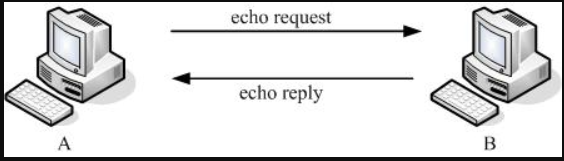
\includegraphics[scale=0.6]{fig1.png}}
\par\par{如果在A主机上能够ping通B主机,那么主机A上显示的信息就是从主机B上返回来的“回显应答”。如果不能ping通,主机A上显示的信息则是由系统自身所产生的错误提示。}


\subsection{Ping程序开发:}
\text{统计ICMP报文结果}
\par{
\begin{lstlisting}
void statistics(int signo){
    printf("\n--------------------PING statistics-------------------\n");
    printf("%d packets transmitted, %d received , %%%d lost\n",nsend,nreceived,
                    (nsend-nreceived)/nsend*100);
    close(sockfd);
    exit(1);
}
\end{lstlisting}
}

\text{校验和算法}
\par{
\begin{lstlisting}
unsigned short cal_chksum(unsigned short *addr,int len)
{
    int nleft=len;
    int sum=0;
    unsigned short *w=addr;
    unsigned short answer=0;

    /*
        The ICMP header binary data is added up in units of 2 bytes.
    */
    while(nleft>1)
    {       sum+=*w++;
            nleft-=2;
    }
    /*
        If the ICMP header has an odd number of bytes, the last byte is left.
        Consider the last byte as the high byte of a 2-byte data,
        the low byte of which is 0, and continue to add
    */
    if( nleft==1)
    {       *(unsigned char *)(&answer)=*(unsigned char *)w;
            sum+=answer;
    }
    sum=(sum>>16)+(sum&0xffff);
    sum+=(sum>>16);
    answer=~sum;
    return answer;
}

\end{lstlisting}
}

\text{设置ICMP报头}
\par{
\begin{lstlisting}
int pack(int pack_no)
{       int i,packsize;
	struct icmp *icmp;
	struct timeval *tval;
	
	icmp=(struct icmp*)sendpacket;
	icmp->icmp_type=ICMP_ECHO;
	icmp->icmp_code=0;
	icmp->icmp_cksum=0;
	icmp->icmp_seq=pack_no;
	icmp->icmp_id=pid;
	packsize=8+datalen;
	tval= (struct timeval *)icmp->icmp_data;
	gettimeofday(tval,NULL);    /*记录发送时间*/
	icmp->icmp_cksum=cal_chksum( (unsigned short *)icmp,packsize); /*校验算法*/
	return packsize;
}

\end{lstlisting}
}

\text{发送3个ICMP报文}
\par{
\begin{lstlisting}
void send_packet()
{       
	int packetsize;
	while( nsend<MAX_NO_PACKETS)
	{       nsend++;
		packetsize=pack(nsend); /*设置ICMP报头*/
		if( sendto(sockfd,sendpacket,packetsize,0,
		(struct sockaddr *)&dest_addr,sizeof(dest_addr) )<0  )
		{       perror("sendto error");
			continue;
		}
		sleep(1); /*每隔一秒发送一个ICMP报文*/
	}
}
\end{lstlisting}
}

\text{两个timeval结构相减}
\par{
\begin{lstlisting}
void tv_sub(struct timeval *out,struct timeval *in)
{       
	if( (out->tv_usec-=in->tv_usec)<0)
	{       --out->tv_sec;
		out->tv_usec+=1000000;
	}
	out->tv_sec-=in->tv_sec;
}
	
\end{lstlisting}
}
\par{接受ICMP报文与剥去报文头部分请详见完整代码。}

\text{主函数部分}
\par{
\begin{lstlisting}
main(int argc,char *argv[])
{       struct hostent *host;
	struct protoent *protocol;
	unsigned long inaddr=0l;
	int waittime=MAX_WAIT_TIME;
	int size=50*1024;
	
	if(argc<2)
	{       printf("usage:%s hostname/IP address\n",argv[0]);
		exit(1);
	}
	
	if( (protocol=getprotobyname("icmp") )==NULL)
	{       perror("getprotobyname");
		exit(1);
	}
	/*生成使用ICMP的原始套接字,这种套接字只有root才能生成*/
	if( (sockfd=socket(AF_INET,SOCK_RAW,protocol->p_proto) )<0)
	{       perror("socket error");
		exit(1);
	}
	/* 回收root权限,设置当前用户权限*/
	setuid(getuid());
	/*扩大套接字接收缓冲区到50K这样做主要为了减小接收缓冲区溢出的
	的可能性,若无意中ping一个广播地址或多播地址,将会引来大量应答*/
	setsockopt(sockfd,SOL_SOCKET,SO_RCVBUF,&size,sizeof(size) );
	bzero(&dest_addr,sizeof(dest_addr));
	dest_addr.sin_family=AF_INET;
	
	/*判断是主机名还是ip地址*/
	if( inaddr=inet_addr(argv[1])==INADDR_NONE)
	{       if((host=gethostbyname(argv[1]) )==NULL) /*是主机名*/
		{       perror("gethostbyname error");
			exit(1);
		}
		memcpy( (char *)&dest_addr.sin_addr,host->h_addr,host->h_length);
	}
	else    /*是ip地址*/
	memcpy( (char *)&dest_addr,(char *)&inaddr,4); //修改host->h_length为4
	/*获取main的进程id,用于设置ICMP的标志符*/
	pid=getpid();
	printf("PING %s(%s): %d bytes data in ICMP packets.\n",argv[1],
	inet_ntoa(dest_addr.sin_addr),datalen);
	send_packet();  /*发送所有ICMP报文*/
	recv_packet();  /*接收所有ICMP报文*/
	statistics(SIGALRM); /*进行统计*/
	
	return 0;
	
}

	
\end{lstlisting}
}

\section{实验结果与分析}
\par{首先给出程序的运行结果:\\}
\subsection{Ping www.baidu.com}
\par\centerline{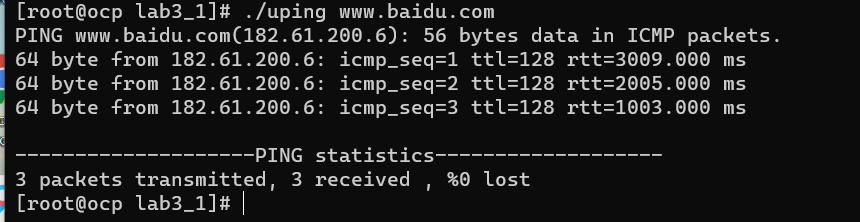
\includegraphics[scale=0.6]{fig2.png}}
\par{从图中可以清楚看到,本程序可以通过主机名顺利Ping通对应的主机,并且输出信息与电脑自带的ping结果相同。(包含IP地址、序列号、RTT延迟等)}
\subsection{Ping 58.192.118.142(东南大学主机地址)}
\par\centerline{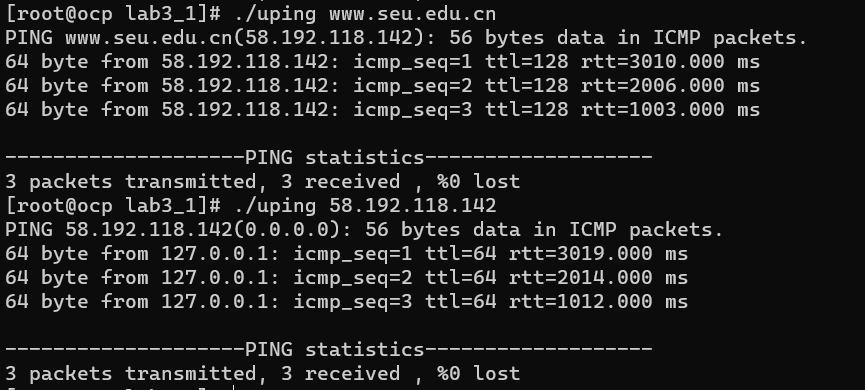
\includegraphics[scale=0.6]{fig3.png}}
\par{我们首先采用Ping主机名的方式,获取www.seu.edu.cn的IP地址,再直接Ping对应的IP地址。}
\subsection{总结}
\par{通过本次实验,首先了解了UDP的通信原理,并且掌握了其C/S结构的程序设计。其次还深入了解了Ping指令的原理。实现了一个自己的Ping程序,并且取得了良好的结果。}
\end{document}
